% Generated by stage1/plot_controls.py; do not edit numerical values here.
% analytic-checks.json SHA-256: 052e4635061b7596c9093604ea3413d86902094092e41997acb327e9e1dba4c4
\subsection{Analytic controls and original-profile audit}
The existing test suite passes 40 tests and 34 subtests
(\path{../results/tests.log}),
including the explicit multimode convolution check with nonzero mean flow.
For plane waves $A=0.6$, $k=0,\pm3$, the largest RHS error is
$1.43\times10^{-12}$ and the largest propagated complex error at
$\xi=2$ is $1.45\times10^{-13}$.
The moving NLS control at $N=2048$, $L=80$, $\mu=2$, $s=1$ has the errors
in Table~\ref{tab:nls}. Successive observed orders approach four
(Figure~\ref{fig:controls}a). Here $p=\log(e_{\rm coarse}/e_{\rm fine})/
\log(h_{\rm coarse}/h_{\rm fine})$; these are exact-solution errors, not
estimates inferred from conservation.

\begin{table}[htbp]
\centering
\caption{Moving NLS complex relative L2 error at $\xi=2$. The ratio compares
with the preceding coarser step.}\label{tab:nls}
\begin{tabular}{rrrr}
\toprule
$\Delta\xi$ & Error & Ratio & Order $p$ \\
\midrule
0.04 & $3.79\times10^{-4}$ & --- & --- \\
0.02 & $2.56\times10^{-5}$ & 14.767 & 3.884 \\
0.01 & $1.65\times10^{-6}$ & 15.548 & 3.959 \\
0.005 & $1.04\times10^{-7}$ & 15.823 & 3.984 \\
\bottomrule
\end{tabular}
\end{table}

A recomputed moving Dysthe profile ($\epsilon=0.025$, $\mu=2$, $s=1$,
$N=4096$, $L=160$) has full residual
$2.06\times10^{-11}$.
At $\xi=2$ and $\Delta\xi=0.000625$,
its raw complex error against the declared traveling solution is
$9.66\times10^{-12}$.

On two independent multimode test fields, full-RHS directional rates of
$\mathcal A,\mathcal M,\mathcal E$ are at most $3.24\times10^{-12}$
in absolute value per unit $\xi$, while the near-cutoff Galerkin energy
rate is $5.92\times10^{-5}$. This explicitly exposes a
projection contribution to invariant drift.


All 28 original stored profiles were independently re-audited on their
original $N=2048$, $L=160$ grid (Figure~\ref{fig:controls}b).
Although every retained residual is at most $4.36\times10^{-11}$,
22 full periodic residuals exceed the current $10^{-8}$ gate.
The largest is $6.12\times10^{-3}$ at
$(\epsilon,\mu,s)=(0.15,3,0)$;
16 profiles also exceed the $\epsilon\max|F|\leq0.1$ design screen.
These results require requalification or finer profile grids; they do not
establish physical instability or nonexistence. The CSV audit retains the
per-profile hashes, residual components, and separate gate decisions.

\begin{figure}[htbp]
\centering
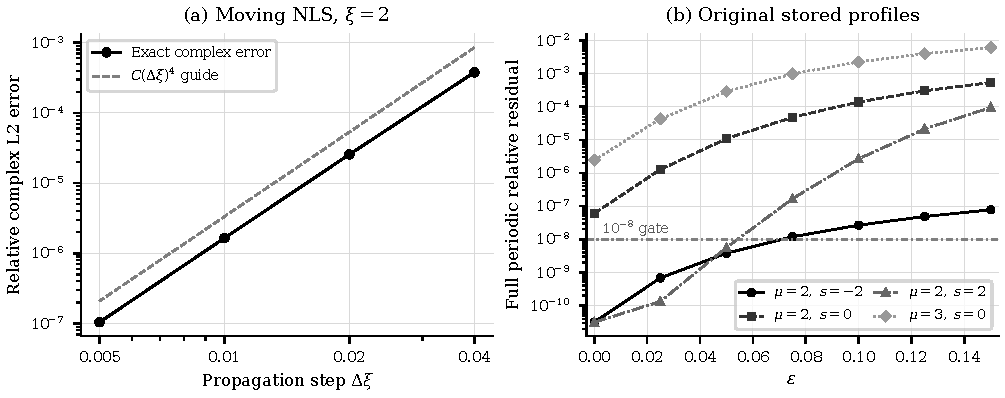
\includegraphics[width=\linewidth]{figures/controls.pdf}
\caption{Analytic propagation control and original-profile full-equation audit.
The dashed fourth-order guide is scaled for visibility. The profile gate
uses the full residual of \eqref{eq:residual}, not the iteration residual.}
\label{fig:controls}
\end{figure}
